\chapter{Fluid Mechanics}
\label{cha:fluid-mechanics}\index{fluid mechanics}
\section{Phase-Space Density}
\label{sec:phase-space-density}
\index{fluid mechanics!phase-space density}
\index{phase-space density}

The phase-space density of particles gives the number of particles in
an infinitesimal region of phase space,
\begin{equation}
d N = f(x^\alpha,{\bf p}) d^3 {\bf x} d^3 {\bf p}
\label{eq:591}
\end{equation}
If there is no dissipation, the phase-space density 
along the trajectory of a particular particle
is given by
\begin{equation}
\dd{f}{\tau} = {\cal C}
\label{eq:592}
\end{equation}
where ${\cal C}$ accounts for two-body interactions between
particles.   This is known as the Boltzmann equation. If there are no collisions, ${\cal C}=0$, so
\index{Lioville's theorem}
\index{fluid mechanics!Lioville's theorem}
\begin{equation}
\dd{f}{\tau} = 0.
\label{eq:593}
\end{equation} 
This is called Lioville's theorem or the collisionless Boltzmann
equation.  This limit applies in galactic dynamics.  Here we are
interested in particles in a gas that do collide so we expand out the
derivative along the flow lines to get
\begin{equation}
\pp{f}{t} + {\bf v} \cdot \nabla f + {\bf F} \cdot \pp{f}{{\bf p}} =
   {\cal C}
\label{eq:594}
\end{equation}
where ${\bf F}$ is a force that accelerates the particles.  The
collision term ${\cal C}$ must now be expressed in the lab frame of
this equation that is no longer manifestly covariant.  The requirement
of no dissipation tells us that $\nabla_{\bf p} \cdot {\bf F} = 0$.

We would like to define some quantities that are integrals over
momentum space that transform simply under Lorentz transformations.
We derived earlier (\S~\ref{sec:transf-radi-transf}) that
\begin{equation}
\frac{d^3 {\bf p}}{p_t} = \frac{d^3{\bf p}'}{p'_t}.
\label{eq:595}
\end{equation}
We also know that $E_{\bf p} = p_t = (p^2 c^2 + m^2 c^4)^{1/2}$
so
\begin{equation}
\frac{d^3 {\bf p}}{E_{\bf p}} = \rmmat{Lorentz Invariant}
\label{eq:596}
\end{equation}
so we can define various integrals
\begin{equation}
\frac{n(x^\alpha)}{{\bar E}_\rmscr{har}(x^\alpha)} \equiv \int \frac{d^3 {\bf
    p}}{E_{\bf p}} f(x^\alpha, {\bf p})
\label{eq:597}
\end{equation}
that transforms as a scalar where $n(x^\alpha)$ is the number density..  Unfortunately, there isn't much that one
can do with it.  One could use it as the source for a scalar theory of
gravity, but it would violate the equivalence principle.

\subsection{Particle Current}
\label{sec:particle-current}
\index{fluid mechanics!particle current}
Next let's define
\begin{equation}
J^\mu (x^\alpha)  \equiv c \int \frac{d^3 {\bf p}}{E_{\bf p}} p^\mu f(x^\alpha, {\bf p}).
\label{eq:598}
\end{equation}
Because this is simply the sum of things that transform as a
four-vector, $J^\mu$ also transforms as a four-vector.  Let's look at
it component by component
\begin{eqnarray}
J^0(x^\alpha) &=& \int \frac{d^3 {\bf p}}{E_{\bf p}} c p^0 f(x^\alpha, {\bf p}) = 
\int d^3 {\bf p} f(x^\alpha, {\bf p}) =  n(x^\alpha) \\
{\bf J}(x^\alpha) &=& \int \frac{d^3 {\bf p}}{E_{\bf p}} c {\bf p}
f(x^\alpha, {\bf p}) = \frac{1}{c} \int d^3 {\bf p} {\bf v} f(x^\alpha, {\bf
  p}) =  \frac{\langle {\bf v} \rangle}{c} n(x^\alpha) 
\label{eq:599}
\end{eqnarray}
If we assume that the scattering (${\cal C}$) conserves energy, momentum
and particles we have
\begin{equation}
J^{\mu}_{~~,\mu} = \pp{J^\mu}{x^\mu} = n \langle \nabla_{\bf p} \cdot {\bf F} \rangle.
\label{eq:600}
\end{equation}
We can prove this simply by integrating Eq.~\ref{eq:594} over $d^3 {\bf p}$.
The first two terms yield the left-hand side of the equation above.  
The third term gives the right-hand side.  This vanishes
as long as 
\begin{equation}
\nabla_{\bf p} \cdot {\bf F} = 0 
\label{eq:601}
\end{equation}
and the right-hand side vanishes if the scattering conserves energy
and momentum.

Let's define ${\bf V}=\langle {\bf v} \rangle$ and write out Eq.~\ref{eq:601}
by components,
\begin{equation}
\pp{n}{t} + \nabla \cdot \left (n {\bf V} \right ) = 0 
\label{eq:602}
\end{equation}
or
\begin{equation}
\pp{\rho}{t} + \nabla \cdot \left (\rho {\bf V} \right ) = 0 
\label{eq:603}
\end{equation}
where $\rho=mn$ where $m$ is the rest mass of the individual particles.
This is the continuity equation.  This must hold true regardless of
the nature of the force, {\em i.e.} even if $\nabla_{\bf p} \cdot F
\neq 0$.  Because Eq.~(\ref{eq:600}) is consistent with the Lioville
equation (Eq.~\ref{eq:593}) and more generally with the Boltzmann
equation (Eq.~\ref{eq:592}) and $J^\mu_{;\mu}=0$ if particles are
conserved,  the Lioville and Boltzmann equations cannot hold if 
$\nabla_{\bf p} \cdot F \neq 0$ and particles are conserved.

\subsection{Stress Tensor}
\label{sec:stress-tensor}
\index{fluid mechanics!stress tensor}

Let's construct a tensor from the distribution function
\begin{equation}
T^{\mu\nu} (x^\alpha)  \equiv c^2 \int \frac{d^3 {\bf p}}{E_{\bf p}}
p^\mu p^\nu f(x^\alpha, {\bf p}).
\label{eq:604}
\end{equation}
this is called the energy-momentum tensor or stress tensor of the
system.  Let's take one of the indices to be zero
\begin{equation}
T^{\mu 0} (x^\alpha) = c^2 \int \frac{d^3 {\bf p}}{E_{\bf p}}
p^\mu \frac{E_{\bf p}}{c} f(x^\alpha, {\bf p}) = 
c \int d^3 {\bf p} p^\mu f(x^\alpha, {\bf p})
\label{eq:605}
\end{equation}
which is the product of the total four momentum of the particle per
unit volume with $c$.  $T^{00}(x^\alpha)$ gives the energy-density and
the component $T^{0\mu}(x^\alpha)$ gives the density of the 
$\mu-$component of the three-momentum.

We are free to fix a Lorentz frame that is moving with the material
such that $J^\mu=0$ for $\mu\neq 0$.  If we are willing to neglect
effects that depend on the gradient of the velocity (such as
viscosity or heat conduction) we can define this frame globally.  Furthermore, let's
assume that the distribution function is isotropic in the momentum.
Fluids for which this is possible are called {\em ideal fluids}.  In
this case we have
\begin{equation}
J^0 = 4\pi \int_0^\infty p^2 f(p) dp, J^\mu = 0 
\label{eq:606}
\end{equation}
and
\begin{equation}
\epsilon = T^{00} = 4\pi \int_0^\infty p^2 E(p) f(p) dp, T^{0\mu}=0
\label{eq:607}
\end{equation}
The space-space part of the energy-momentum tensor must be symmetric,
isotropic and a three-dimensional tensor (a matrix).  The only tensor
that works is
\begin{equation}
T^i_{~~j} = P \delta^i_{~~j}
\label{eq:608}
\end{equation}
where
\begin{equation}
T^i_{~~i} = P \delta^i_{~~i} = 3 P = c^2 \int \frac{d^3 {\bf p}}{E_p} p^2 f(p) = 
4 \pi c^2 \int_0^\infty \frac{p^4}{E(p)} f(p) dp
\label{eq:609}
\end{equation}
so
\begin{equation}
P = \frac{4 \pi}{3} c^2 \int_0^\infty \frac{p^4}{E(p)} f(p) dp.
\label{eq:610}
\end{equation}
Notice that the trace of the energy-momentum tensor $T^\mu_{~~\mu}$ is a
scalar.  In fact it is simply the product of $m^2 c^4$ with the scalar
density defined in Eq.~\ref{eq:597}.

Let's look at the non-relativistic limit of the energy-momentum tensor.
Let's take $T^{00} = mc^2 n + \epsilon_\rmscr{nr}$ where
\begin{equation}
T^{00} = 4\pi \int_0^\infty p^2 \left (mc^2 + \frac{p^2}{2m} \right )
f(p) dp = n mc^2 + \epsilon_\rmscr{nr}
\label{eq:611}
\end{equation}
where
\begin{equation}
\epsilon_\rmscr{nr} = 4\pi \int_0^\infty p^2 \frac{p^2}{2m} f(p) dp =
\frac{2\pi}{m} \int_0^\infty p^4 f(p) dp.
\label{eq:612}
\end{equation}
Let's look at the non-relativistic limit of the pressure
\begin{equation}
P_\rmscr{nr} = \frac{4 \pi}{3} c^2 \int_0^\infty \frac{p^4}{mc^2}
f(p) = \frac{4\pi}{3m} \int_0^\infty p^4 f(p) dp
\label{eq:613}
\end{equation}
so $\epsilon_\rmscr{nr} = \frac{3}{2} P_\rmscr{nr}$.  Now let's take
the opposite limit
\begin{equation}
\epsilon_\rmscr{ur} = T^{00} = 4 \pi \int_0^\infty p^2 (p c) f(p) dp,
p_\rmscr{ur} = \frac{4\pi}{3} c^2 \int_0^\infty \frac{p^4}{pc} f(p) dp
\label{eq:614}
\end{equation}
so $P=\epsilon/3$ in the ultrarelativistic limit.  We can transform
from this special frame to a frame where the fluid moves and get
\begin{equation}
T^\mu_{~~\nu} = (P + \epsilon) U^\mu U_\nu - P \delta^\mu_{~~\nu}
\label{eq:615}
\end{equation}
and 
\begin{equation}
J^\mu = n_\rmscr{prop} U^\mu
\label{eq:616}
\end{equation}
$n_\rmscr{prop}$ is the number density of the particles in a frame
moving with the particles and $U^\mu$ is the bulk four-velocity of the
fluid. 

We can calculate the evolution of this tensor by integrating over
Lioville's equation times $p^\mu$ to get
\begin{equation}
T^{\mu\nu}_{~~~~,\nu} = \pp{T^{\mu\nu}}{x^\nu} = \left \{ \begin{array}{ll}
n \langle {\bf v} \cdot {\bf F} \rangle, & \mu = 0 \\
c n \langle {\bf F} \rangle, & \mu > 0 
\end{array} \right . .
\label{eq:617}
\end{equation}
We prove this by integrating Eq.~\ref{eq:594} times $p^\mu$ over $d^3{\bf p}$.
The zero-component is simply the work performed by the force on the
particles in the volume.  The other components account for the change
in the momentum of the particles.

\paragraph{Non-relativistic limit}
\label{sec:non-relat-limit}
\index{fluid mechanics!non-relativistic}\\

Let's examine what this equation means in the non-relativistic limit,
\begin{equation}
T^{00} = c^2 \int d^3 {\bf p} f(p) m c^2 \left ( 1 +
\frac{1}{2}\frac{v^2}{c^2} \right )= \rho c^2 + \int d^3 p f \left (
\frac{1}{2} m v^2 \right ) = \rho c^2 + n \langle E \rangle
\label{eq:618}
\end{equation}
and
\begin{equation}
T^{0\nu} = c^2 \int d^3 {\bf p} f m c v^\nu \left ( 1 +
\frac{1}{2}\frac{v^2}{c^2}\right ) = \left ( \rho c {\bf V} +
\frac{1}{c} {\bf q} \right )^{\nu}
\label{eq:619}
\end{equation}
where
\begin{equation}
{\bf q} = \int d^3 {\bf p} \left ( \frac{1}{2} m v^2 \right ) {\bf v} f
\label{eq:620}
\end{equation}
is the flux of kinetic energy.  The first term is the flux of
rest-mass energy.  Finally for the space-space part we have
\begin{equation}
T^{\mu\nu} = \int d^3{\bf p} m v^\mu v^\nu f.
\label{eq:621}
\end{equation}
Let's look at the zero-component of Eq.~\ref{eq:617} 
\begin{equation}
\frac{1}{c} \pp{}{t} \left ( \rho c^2 + n \langle E \rangle \right ) + \nabla
\cdot \left ( \rho c {\bf V} + \frac{\bf q}{c} \right ) = n \langle
      {\bf v} \cdot {\bf F} \rangle
\label{eq:622}
\end{equation}
We can subtract $c$ times the continuity equation to get
\begin{equation}
\pp{n \langle E \rangle}{t} + \nabla \cdot {\bf q} = n \langle
      {\bf v} \cdot {\bf F} \rangle.
\label{eq:623}
\end{equation}
This ensures conservation of energy.  We can divide the energy from
the bulk flow from the random kinetic energy of the fluid
\begin{equation}
N \langle E \rangle = N \left \langle \frac{1}{2} m \left ( {\bf V} + {\bf v}_r
\right )^2 \right \rangle = \frac{1}{2} \rho V^2 + \frac{1}{2} \rho
\langle v_r^2 \rangle = \frac{1}{2} \rho V^2 + \frac{3}{2} N T,
\label{eq:624}
\end{equation}
defining the temperature $T$ of the fluid.

The spatial part of Eq.~\ref{eq:618} gives
\begin{equation}
\frac{1}{c} \pp{}{t} \left ( \rho c {\bf V} + \frac{\bf q}{c} \right
)^i + \pp{T^{ik}}{x^k} = n \langle {\bf F} \rangle.
\label{eq:625}
\end{equation}
The first term in the parentheses is larger by a factor of $c^2$ so to
lowest order we have
\begin{equation}
\pp{}{t} \left ( \rho V^i \right ) + \pp{T^{ik}}{x^k} = n \langle {\bf F} \rangle.
\label{eq:626}
\end{equation}
This is equivalent to neglecting the momentum carried by the flow of 
energy.

\section{Ideal Fluids}
\label{sec:ideal-fluids}
\index{fluid mechanics!ideal fluids}
\index{ideal fluids}
For an ideal fluid we found that the stress tensor took a particular
form,
\begin{equation}
T^{\mu\nu} = (p + \epsilon) U^\mu U^\nu - P g^{\mu\nu}
\label{eq:627}
\end{equation}
In the non-relativistic limit we find that space-space components are
\begin{equation}
T_{ik} = \rho V_i V_k + P \delta_{ik}
\label{eq:628}
\end{equation}
and
\begin{equation}
{\bf q} = \left [ \frac{1}{2} V^2 + w \right ] \rho {\bf V}
\label{eq:629}
\end{equation}
where $w=(\epsilon + P)/\rho$ is the heat function (enthalpy) per
unit mass of the fluid. Notice that there is no energy flow without
bulk motion.  If we substitute this into the equations
derived earlier we get
\begin{equation}
\pp{\rho}{t} + \nabla \cdot \left ( \rho {\bf V} \right ) = 
\pp{\rho}{t} + \left ( {\bf V} \cdot \nabla \right ) \rho 
+ \rho \nabla \cdot {\bf V} =
\dd{\rho}{t} + \rho \nabla \cdot {\bf V} = 0
\label{eq:630}
\end{equation}
and
\begin{equation}
\pp{{\bf V}}{t} + \left ( {\bf V} \cdot \nabla \right ) {\bf V} =
\dd{\bf V}{t} = -\frac{\nabla P}{\rho} + \frac{\langle {\bf F} \rangle}{m}
\label{eq:631}
\end{equation}

In the ideal fluid, no heat is tranferred between different parts of
the fluid, so if we denote $s$ as the entropy per unit rest mass we have
\begin{equation}
\dd{s}{t} = 0
\label{eq:632}
\end{equation}
for a bunch of fluid; therefore, we also have a continuity equation
for the entropy
\begin{equation}
\pp{(\rho s)}{t} + \nabla \cdot \left ( \rho s {\bf v} \right ) = 0.
\label{eq:633}
\end{equation}
We can use the continuity equation for particle number to simplify
this further,
\begin{equation}
\rho \pp{s}{t} + {\bf v} \cdot \nabla (\rho s) = 0.
\label{eq:634}
\end{equation}

\subsection{Isentropic flows}
\label{sec:isentropic-flows}
\index{fluid mechanics!isentropic flows}
\index{isentropic flows}

An important case of adiabatic flows is when the entropy $s$ is
initially constant.  In such an isentropic flow, the entropy will
remain constant and we can derive some additional useful forms of
Eq.~\ref{eq:631}.

From the definition of the work function $w$ and thermodynamics we
know that
\begin{equation}
d w = T ds + \frac{1}{\rho} dp = \frac{dp}{\rho}
\label{eq:635}
\end{equation}
because the entropy is constant, $ds=0$.  We get
\begin{equation}
\pp{{\bf V}}{t} + \left ( {\bf V} \cdot \nabla \right ) {\bf V} =
\dd{\bf V}{t} = -\nabla w + \frac{\langle {\bf F} \rangle}{m}
\label{eq:636}
\end{equation}
From vector analysis we know
\begin{equation}
\frac{1}{2} \nabla v^2 = {\bf v} \times (\nabla \times {\bf v}) + ({\bf
  v} \cdot \nabla ) {\bf v}
\label{eq:637}
\end{equation}
and we can get
\begin{equation}
\pp{{\bf V}}{t} + \frac{1}{2} \nabla v^2 - {\bf v} \times (\nabla
\times {\bf v} ) = -\nabla w + \frac{\langle {\bf F} \rangle}{m}.
\label{eq:638}
\end{equation}
If we take the curl of both sides we find that
\begin{equation}
\pp{}{t}\left ( \nabla \times {\bf V} \right ) = \nabla \times \left( {\bf V}
\times (\nabla \times {\bf V} ) \right ) + \nabla \times \frac{\langle
  {\bf F} \rangle }{m}
\label{eq:639}
\end{equation}
$\omega = \nabla \times {\bf V}$ is called the vorticity.

If we assume that ${\bf F}/m = -\nabla \phi$ which is often the case,
we find that if the flow in an isentropic, ideal fluid is initially
irrotational it will remain irrotational.

We can go further than this.  Let's define
\begin{equation}
\Gamma = \oint {\bf v} \cdot d{\bf l}
\label{eq:640}
\end{equation}
taken along some closed contour that moves with the fluid.   Let's
calculate
\begin{equation}
\dd{\Gamma}{t} = \dd{}{t}\oint {\bf v} \cdot d{\bf l} = \dd{}{t} \oint {\bf v}
\cdot \delta {\bf r} = \oint \dd{\bf v}{t} \cdot \delta {\bf r}
+ \oint {\bf v} \cdot \dd{}{t} \delta {\bf r}.
\label{eq:641}
\end{equation}
Because $\delta {\bf r}$ is the difference between two positions
moving with the fluid we have
\begin{equation}
{\bf v} \cdot \dd{}{t} \delta {\bf r} = {\bf v} \cdot \delta \dd{\bf
  r}{t} = {\bf v} \cdot \delta {\bf v} = \delta v^2
\label{eq:642}
\end{equation}
so
\begin{equation}
\dd{}{t}\oint {\bf v} \cdot d{\bf l} =\oint \dd{\bf v}{t} \cdot d {\bf
  l} = \oint \left ( -\nabla w + \frac{\langle {\bf F} \rangle}{m}
\right ) d {\bf l} = 0 
\label{eq:643}
\end{equation}
if ${\bf F}/m = -\nabla \phi$, so the circulation around a contour
moving with the fluid is constant if the flow is isentropic.

\begin{figure}
\begin{center}
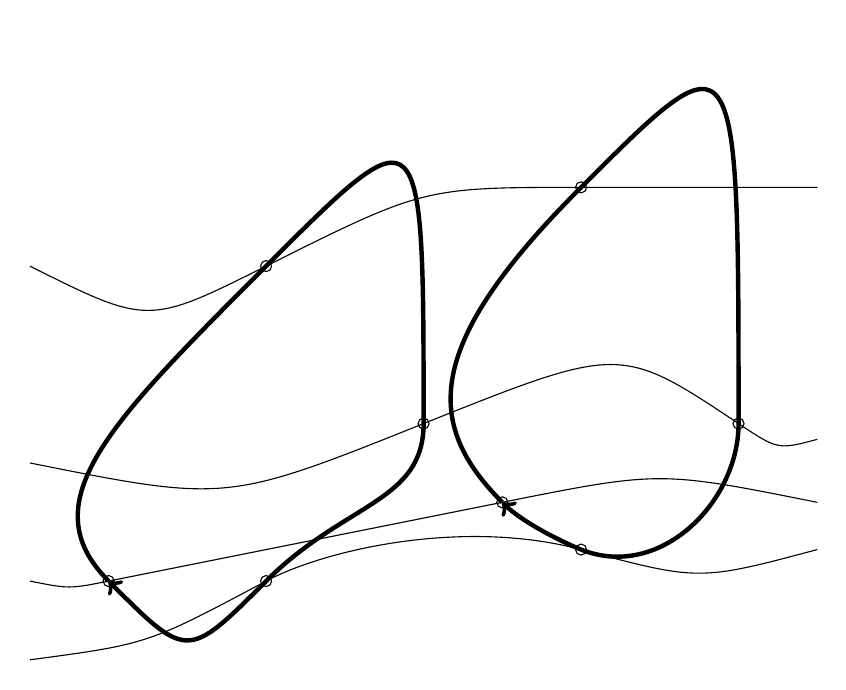
\begin{tikzpicture}
\draw [->,ultra thick] (0,0) .. controls (-1,1) and (0,2) .. (2,4) .. controls (4,6)
.. (4,2) .. controls (4,1) and (3,1) .. (2,0) .. controls (1,-1)
.. (0,0);
\draw [->,ultra thick] (5,1) .. controls (4,2) and (4,3) .. (6,5) .. controls (8,7)
.. (8,2) .. controls (8,1) and (7,0) .. (6,0.4) .. controls (5.75,0.5)
and (5.25,0.75) .. (5,1);
\draw [->] (-1,0) .. controls (-0.5,-0.1) .. (0,0) circle (2pt)
.. controls (0.5,0.1) .. (5,1) circle (2pt) .. controls (7,1.4) .. (9,1);
\draw [->] (-1,4) .. controls (0.5,3.25) .. (2,4) circle (2pt)
.. controls (4,5) .. (6,5) circle (2pt) -- (9,5);
\draw [->] (-1,1.5) .. controls (1.5,1) .. (4,2) circle (2pt)
.. controls (6.5,3) .. (8,2) circle (2pt) .. controls (8.5,1.66667) .. (9,1.8);
\draw [->] (-1,-1) .. controls (0.5,-0.8) .. (2,0) circle (2pt)
.. controls (2.75,0.4) and (4.5,0.8) .. (6,0.4) circle (2pt) .. controls (7.5,0) .. (9,0.4);
\end{tikzpicture}
\caption{The circulation around a close contour (bold lines) that
  travels with the fluid along the streamlines (light lines) is
  conserved if the fluid is isentropic.}
\end{center}
\end{figure}

\subsection{Hydrostatics}
\label{sec:hydrostatics}
\index{fluid mechanics!hydrostatics}
\index{hydrostatics}
Let's assume that the fluid is not moving.  If we look at Eq.~\ref{eq:632} we
get the equation of hydrostatic equilibrium.  Let's further suppose
that the force is derived from a potential, we obtain,
\begin{equation}
\frac{\nabla P}{\rho} = - \nabla \phi.
\label{eq:644}
\end{equation}
Let's take the divergence of both sides
\begin{equation}
\nabla \cdot \left ( \frac{\nabla p}{\rho} \right ) = -\nabla^2 \phi
= -4\pi G \rho
\label{eq:645}
\end{equation}
and in spherical coordinates we have
\begin{equation}
\frac{1}{r^2} \dd{}{r} \left ( \frac{r^2}{\rho} \dd{p}{r} \right ) =
-4\pi G \rho.
\label{eq:646}
\end{equation}
An interesting and important case is when the fluid is isentropic as
well, then we have
\begin{equation}
\nabla w = -\nabla \phi.
\label{eq:647}
\end{equation}
and
\begin{equation}
\nabla^2 w = -4\pi G \rho
\label{eq:648}
\end{equation}
If we look at the Eq.~\ref{eq:648} and imagine that the fluid is rotating we
have an extra term,
\begin{equation}
\nabla w = -\nabla \phi + \Omega^2({\bf r}) {\bf R}
\label{eq:649}
\end{equation}
where ${\bf R}$ is a vector pointing from the rotation axis to 
the point in the fluid.  Let's take the curl of both sides to get
\begin{equation}
0 = 0 + \nabla \times \left ( \Omega^2({\bf r}) {\bf R} \right )
\label{eq:650}
\end{equation}
which tells us that
\begin{equation}
\Omega ( {\bf r} ) = \Omega(R)
\label{eq:651}
\end{equation}
or that isentropic stars must have constant angular velocity on
cylindrical surfaces.

\subsection{Really Little Sound Waves}
\label{sec:really-little-sound}
\index{sound waves}
\index{fluid mechanics!sound waves}
The next order of complexity is to assume that the fluid is at rest
with a small perturbation and to see what the perturbation does.  We
have 
\begin{equation}
\pp{\rho}{t} + \nabla \cdot (\rho {\bf V}) = \pp{\rho'}{t} + \rho_0
\nabla \cdot {\bf V}' = 0 
\label{eq:652}
\end{equation}
and 
\begin{equation}
\pp{{\bf V}}{t} + \left ( {\bf V} \cdot \nabla \right ) {\bf V} =
\dd{\bf V}{t} + \frac{\nabla P}{\rho} =
\pp{{\bf V}'}{t} + \frac{\nabla P'}{\rho_0} = 0.
\label{eq:653}
\end{equation}
We can write $P' = (\partial P/\partial \rho)_s \rho'$ and rewrite the
continuity equation to get
\begin{equation}
\pp{P'}{t} + \rho_0 \left ( \pp{P}{\rho} \right )_s \nabla \cdot {\bf
  V'} = 0
\label{eq:654}
\end{equation}
Let's take the divergence of the Euler equation to get
\begin{equation}
\pp{{\bf \nabla \cdot V}'}{t} + \frac{\nabla^2 P'}{\rho_0} = 0.
\label{eq:655}
\end{equation}
and the time derivative of the continuity equation to get
\begin{equation}
\pp{^2 P'}{t^2} + \rho_0 \left ( \pp{P}{\rho} \right )_s \nabla \cdot \pp{\bf
  V'}{t} = 0.
\label{eq:656}
\end{equation}
Finally we put the two together to get
\begin{equation}
\pp{^2 P'}{t^2} - \left ( \pp{P}{\rho} \right )_s \nabla^2 P' = 0.
\label{eq:657}
\end{equation}
This is a wave equation with a sound speed of $c_s^2 = (\partial
P/\partial \rho)_s$.  Let's take a solution to this equation for the
pressure,
\begin{equation}
P' = p' \exp[i({\bf k} \cdot {\bf r} - \omega t)]
\label{eq:658}
\end{equation}
with $k^2 c_s^2=  \omega^2$ and calculate the velocity of the fluid
\begin{equation}
{\bf V}' = {\bf v}' \exp[i({\bf k} \cdot {\bf r} - \omega t)]
\label{eq:659}
\end{equation}
From Eq.~\ref{eq:654} we get
\begin{equation}
- \omega {\bf v}' +  \frac{p'}{\rho_0} {\bf k} = 0
\label{eq:660}
\end{equation}
and from Eq.~\ref{eq:655} we get
\begin{equation}
- \omega p' +  \rho_0 c_s^2 {\bf k} \cdot {\bf v'} = 0.
\label{eq:661}
\end{equation}
Combining these results gives
\begin{equation}
- \omega {\bf v}' +  \frac{c_s^2 {\bf k} \cdot {\bf
    v'}}{\omega} {\bf k} =0
\label{eq:662}
\end{equation}
and rearranging
\begin{equation}
{\bf v}' = \frac{c_s^2 {\bf k} \cdot {\bf v'}}{\omega^2} {\bf
  k} = v' \frac{\bf k}{k}.
\label{eq:663}
\end{equation}
Therefore, the fluid is displaced in the direction of the propagation
of the wave; it is a longitudinal wave.

\subsection{Steady Supersonic Flow}
\label{sec:steady-supers-flow}
\index{fluid mechanics!supersonic flow}
\index{supersonic flow}
Many disturbances travel through a fluid at a finite speed (changes in
the entropy or vorticity move with the fluid).  If the fluid itself
travels faster than the speed of sound, a disturbance starting at
particular point only can travel downstream so the upsteam flow cannot
know about it.  A flow can become supersonic abruptly as in a
shock or continuously.  We will examine this latter case here.

Let's imagine that a fluid is flowing through a pipe of variable cross
section $A(x)$ and that the flow is steady so that all partial time
derivatives vanish.  We can write the continuity equation as $\rho v
A=$constant.  The Euler equation becomes
\begin{equation}
v \dd{v}{t} = - \frac{1}{\rho} \dd{p}{t} = -\frac{c_s^2(\rho)}{\rho} \dd{\rho}{t}
\label{eq:664}
\end{equation}
where we have assumed that the fluid flows in the $x-$direction.  From
the continuity equation we know
\begin{equation}
-\frac{1}{A} \dd{A}{t} = \frac{1}{\rho v} \dd{(\rho v)}{t} 
= \frac{1}{\rho v} \left ( v \dd{\rho}{t} + \rho \dd{v}{t}  \right ) .
\label{eq:665}
\end{equation}
We can combine the two equations to get
\index{fluid mechanics!de Laval nozzle}
\index{de Laval nozzle}
\begin{equation}
\dd{\ln A}{t} = \frac{c_s^2}{v^2} \left ( 1 -
\frac{v^2}{c_s^2} \right ) \dd{\ln \rho}{t} = \frac{p}{\rho v^2}  \left ( 1 -
\frac{v^2}{c_s^2} \right )\dd{\ln p}{t} = - \left ( 1 -
\frac{v^2}{c_s^2} \right ) \dd{\ln v}{t}.
\label{eq:deLaval}
\label{eq:666}
\end{equation}
If $v<c_s$ we have the following situation,
\begin{itemize}
\item If the area of the pipe decreases (nozzle) in the direction of
  the flow, the velocity increases and the pressure and density
  decrease.
\item If the area of the pipe increases (diffuser) in the direction 
  of the flow,  the velocity decreases and the pressure and density increase.
\end{itemize}
On the other hand if the flow is supersonic ($v>c_s$) we have
\begin{itemize}
\item If the area of the pipe decreases (nozzle) in the direction of
  the flow, the velocity decreases and the pressure and density
  increase.
\item If the area of the pipe increases (diffuser) in the direction 
  of the flow,  the velocity increases and the pressure and density 
  decrease.
\end{itemize}

If we have a tube in which the flow is initially subsonic and the area
of the tube decreases, the flow will accelerate.  If the area of the
tube increases again the flow will decelerate and you're back where
you started.   On the other hand let's imagine that the area of the
tube decreases sufficiently that the velocity of the flow reaches the
speed of sound at the cinch point of the tube, the fluid will exit the
cinch point supersonically and accelerate as the tube inreases in
cross-section.   Now you know why a rocket engine is shaped like it is
(this is called a de Laval nozzle).


%\subsection{Bigger Sound Waves}
%
%Let's revisit sound waves but this time we will treat their evolution
%exactly rather than pertubatively.  The wave is
%travelling in the $x-$direction so we have the continuity and Euler
%equation
%\begin{equation}
%\pp{\rho}{t} + \pp{(\rho v)}{x} = 0, \pp{v}{t} + v \pp{v}{x} +
%\frac{1}{\rho} \pp{p}{x} = 0.
\label{eq:667}
%\end{equation}
%Let's assume that the flow is adiabatic so $p=p(\rho)$ and also let's
%assume that the velocity of the fluid is function of density alone
%$v=v(\rho)$, then we have
%\begin{equation}
%\pp{\rho}{t} + \dd{(\rho v)}{\rho} \pp{\rho}{x} = 0, \pp{v}{t} + \left
%( v + \frac{1}{\rho} \dd{p}{v} \right ) \pp{v}{x} = 0
\label{eq:668}
%\end{equation}
%

\subsection{Flow through a Channel}
\label{sec:flow-through-channel}
{
\begin{figure}
\begin{center}
\begin{tikzpicture}
\draw [scale=5] plot file {channel_dat/chan_y.res} node [right] {$y(x)$}
                plot file {channel_dat/chan.res} node [right] {$z(x)$}
                plot file {channel_dat/chan_m.res}
                plot file {channel_dat/chan_t.res};
\foreach \y in {1,...,4} \draw [->] (-4,\y) -- (-2.5,\y);
\draw (-2.5,4) node [right] {$v(x)$};
\end{tikzpicture}
%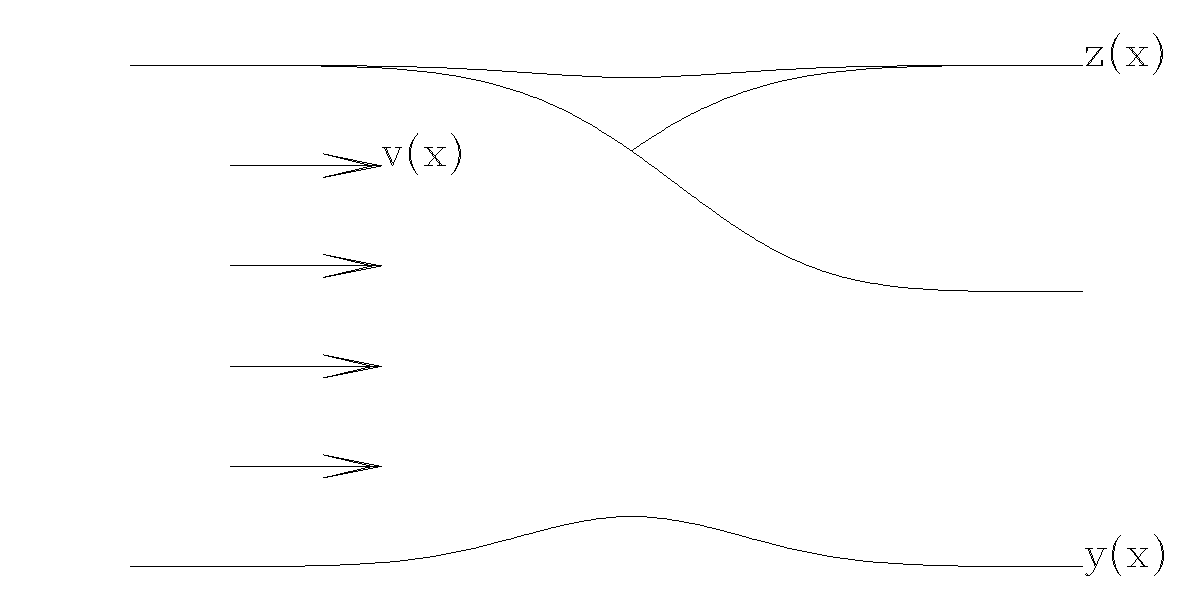
\includegraphics[width=\textwidth]{channel} 
\caption{A channel of variable depth}
\label{fig:channel}
\end{center}
\end{figure}


We can see many of the features of the supersonic flow through a de
Laval nozzle in the flow through a channel.  Much of the intuition
developed in hydraulics carries over to other fluid systems (even
astrophysical ones); furthermore, water running through a channel is
something with which most are familiar.

Let's look at a channel of constant width but varying depth $y(x)$.
Let's take $y$ equals to zero well before the bump.  We would like to
know how the height of the surface of the flow $z(x)$ changes as it
passes through the channel (as shown in Fig.~\ref{fig:channel}).

Let's write out the Bernoulli equation (divided by $g$ as customary in
hydraulics) for the fluid moving along the
surface,
\begin{equation}
\frac{v^2}{2g} + z + \frac{p_a}{g}= \frac{v_0^2}{2g} + z_0 +
\frac{p_a}{g} = h_0
\label{eq:669}
\end{equation}
where $p_a$ is the pressure of the atmosphere.  The quantity $h_0$ is
a constant along the surface streamline, and it is so important in
hydraulics that it has a special name, {\em specific head}.
From continuity we have
\begin{equation}
v \left ( z - y \right ) = v_0 z_0 = q_0
\label{eq:670}
\end{equation}
where $q_0$ is the flux.  Notice that we have neglected
the vertical velocity of the flow.  This is a common assumption in
hydraulics.  Combining the equations yields
\begin{equation}
\frac{v_0^2}{2} \left [ \left ( \frac{z_0}{z-y} \right )^2 - 1 \right
] + g \left (z-z_0\right) = 0 .
\label{eq:bern}
\label{eq:671}
\end{equation}
Taking the derivative with respect to $x$ yields
\begin{equation}
\frac{dy}{dx}=\frac{dz}{dx} \left [ 1 - \frac{g\left(z-y\right)^{3}}{v_0^2
      z_0^2} \right ] = \frac{dz}{dx} \left [ 1 -
    \frac{g\left(z-y\right)}{v^2} \right ] = 
\frac{dz}{dx} \left [ 1 - \mathrm{Fr}^{-2}\right ].
\label{eq:672}
\end{equation}
where $\mathrm{Fr}$ is the Froude number, the ratio of the speed of
flow to the speed of small wavelength gravity waves (see
\S~\ref{sec:gravitywaves}).  We can rearrange this a bit to yield
\begin{equation}
\frac{dz}{dx} = -\frac{dy}{dx} \frac{\mathrm{Fr}^2}{1-\mathrm{Fr}^2},
\label{eq:dzdx}
\label{eq:673}
\end{equation}
so if the fluid is {\em subcritical} or streaming (``subsonic'') over the bump, the surface will dip, and 
if the fluid is {\em supercritical} or shooting (``supersonic'') the surface will bulge.  For the
equation to make sense, if the flow becomes supercritical, it must do
so at the top of the bump.  

Fig.~\ref{fig:channel} shows the various possibilities.  Essentially
for given values of $g, v_0$ and $z_0$ and for a small enough values
of $y(x)$, there are two solutions for $z(x)$.  One is a small
deviation in the level of the surface that corresponds to a subcritical
flow.  The second has a large deviation (supercritical flow).  When the
flow is critical these two solutions coincide.  The upper curves show the
surface for various values of $v_0$.  The uppermost curve is always
well in the subcritical regime.  The middle curve nearly reaches the
critical point at the top of the bump, and the lower curve reaches the
critical point and is supercritical to the right of the bump.

When the flow is critical at the top of the bump, we see that the
smooth solution is the one that goes supercritical after the bump.  At
first glance the whole setup seems quite sensitive.  In particular
what if the bump is so big that the flow goes critical before reaching
the top of the bump?  For a particular set of initial conditions we
can calculate the height of the bump where the fluid goes
critical to be
\begin{equation}
y_c = z_0 + \frac{v_0^2}{2g} - \frac{3 \left (v_0 z_0\right)^{2/3}}{2
  g^{1/3}} = h_0 - \frac{3 q_0^{2/3}}{2 g^{1/3}}
\label{eq:ycrit}
\label{eq:674}
\end{equation}
We can actually do much better than this.  If we look at
Eq.~\ref{eq:bern} and make the substitution $z=y+1/u$ we get
\begin{equation}
\frac{v_0^2 z_0^2}{2} u^3 - \left [ \frac{v_0^2}{2} + g \left ( z_0 -
    y \right )   \right ] u + g = 0.
\label{eq:bernu}
\label{eq:675}
\end{equation}
This equation has the form
\begin{equation}
A u^3 - B u + C = 0.
\label{eq:cubic}
\label{eq:676}
\end{equation}
\index{cubic equation}
Let us substitute $u=\sqrt{4B/3A} \cos t$ to give after some
manipulation
\begin{equation}
\cos 3 t = -\frac{3 C}{2 B} \sqrt{\frac{3A}{B}}
\label{eq:cubic_sol}
\label{eq:677}
\end{equation}
which gives three real solutions for $u$ as long as the absolute value
of the right-hand side does not exceed unity.
We can also use this result to solve for $v_0$ in terms of $y_c$ in
Eq.~\ref{eq:ycrit}.   Both this and the solutions to
Eq.~\ref{eq:bernu} are left for the exercises.


\section{Real Sound Waves}
\label{sec:real-sound-waves}
\index{fluid mechanics!sound waves}
Let's take a closer look at sound waves.  As before we shall assume
that the background is static so before we perturb the medium the
entropy is constant throughout.  Let's perturb the fluid in a
particular wave so that $s$ remains constant.  In this case, we can
express the pressure in terms of the density alone.

Furthermore, let's assume that the velocity of fluid at any point depends
on the density alone and look at the continuity and Euler equations
\begin{equation}
\pp{\rho}{t} + \pp{(\rho v)}{x} = 0, ~~~ \pp{v}{t} + v \pp{v}{x} +
\frac{1}{\rho} \pp{P}{x} = 0
\label{eq:680}
\end{equation}
where we have assumed that the wave is a plane wave travelling in the
$x-$direction.  Using the relationships between the pressure, velocity
and density we can obtain,
\begin{equation}
\pp{\rho}{t} + \dd{(\rho v)}{\rho} \pp{\rho}{x} = 0, ~~~ \pp{v}{t} +
\left ( v + \frac{1}{\rho} \dd{P}{v} \right ) \pp{v}{x} = 0.
\label{eq:681}
\end{equation}
We can define the speed of the wave as the rate at which regions of
the same density or velocity move forward along the $x-$direction,
\begin{equation}
\left( \pp{x}{t} \right )_\rho = - \left [
  \frac{\pp{\rho}{t}}{\pp{\rho}{x}} \right ] = \dd{(\rho v)}{\rho} = v
+ \rho \dd{v}{\rho}
\label{eq:682}
\end{equation}
and
\begin{equation}
\left( \pp{x}{t} \right )_v = - \left [
  \frac{\pp{v}{t}}{\pp{v}{x}} \right ] = v + \frac{1}{\rho} \dd{P}{v}.
\label{eq:683}
\end{equation}
These two velocities must be equal so we get
\begin{equation}
\rho \dd{v}{\rho} = \frac{1}{\rho} \dd{P}{v} = \frac{c_s^2}{\rho} \dd{\rho}{v}
\label{eq:684}
\end{equation}
so
\begin{equation}
v = \pm \int \frac{c_s}{\rho} d\rho = \pm \int \frac{dP}{\rho c_s}.
\label{eq:685}
\end{equation}
We can find how fast a portion of the wave travels by substituting
into Eq.~\ref{eq:684} to get
\begin{equation}
\left( \pp{x}{t} \right )_v = v \pm c_s(v)
\label{eq:686}
\end{equation}
so we find that
\begin{equation}
x = t [  v \pm c_s(v) ] + f(v)
\label{eq:687}
\end{equation}
where $f(v)$ determines the initial shape of the wave.   Let's derive
an expresion for the sound speed as a function of the density,
\begin{equation}
c_s = \left [\dd{P}{\rho}\right ]^{1/2} = \left [ \gamma K
  \rho^{\gamma-1} \right ]^{1/2}
\label{eq:688}
\end{equation}
so
\begin{equation}
\rho = \rho_0 \left ( \frac{c_s}{c_0} \right )^{2/(\gamma-1)}.
\label{eq:689}
\end{equation}
If we substitute this into Eq.~\ref{eq:688} we get
\begin{equation}
c_s = c_0 \pm \frac{1}{2} (\gamma -1 ) v.
\label{eq:690}
\end{equation}
We can use this result to express the density and pressure in terms of
the fluid velocity
\begin{equation}
\rho = \rho_0 \left [ 1 \pm \frac{1}{2} (\gamma-1) \frac{v}{c_0}
  \right]^{2/(\gamma-1)}, ~~~ P = P_0
\left [ 1 \pm \frac{1}{2} (\gamma-1) \frac{v}{c_0}
  \right]^{2\gamma/(\gamma-1)}.
\label{eq:691}
\end{equation}
Putting things together we find that
\begin{equation}
x = t \left [ \pm c_0 + \frac{1}{2} (\gamma+1) v \right ] + f(v)
\label{eq:692}
\end{equation}
or rearranging
\begin{equation}
v = F \left \{ x - \left [ \pm c_0 + \frac{1}{2} (\gamma+1) v \right ]
t \right \}
\label{eq:693}
\end{equation}
If we look at Eq.~\ref{eq:693} we see that we can have a situation where the
same value of $x$ has more than one value of $v$.  This isn't
physical.  This first occurs at a time $t$ when
\begin{equation}
\left ( \pp{x}{v} \right)_t = 0, \left ( \pp{^2x}{v^2} \right)_t = 0, 
\label{eq:694}
\end{equation}
or at
\begin{equation}
t = -\frac{2 f'(v)}{\gamma+1}, f''(v) = 0.
\label{eq:695}
\end{equation}
\index{fluid mechanics!shock formation}
The first expression tells us when the shock forms, and the second
tells us that the shock forms at a point of inflection in the wave.

Another important situation is when the discontinuity forms at a
boundary between gas that is moving at gas that is stationary
($v=0$).  In this case we have
\begin{equation}
t = - \frac{2f'(0)}{\gamma+1}
\label{eq:696}
\end{equation}
As an example let's assume that we have a pipe closed at one end by a
piston and we start to move the piston according to $v_\rmscr{pist}=a
t$.  Because the gas at the edge of the piston must move with the
piston we have $v=at$ at $x=\frac{1}{2} at^2$, so we can write down an
expression for 
\begin{equation}
f(v) = f(at) = \frac{1}{2} at^2 - -c_0 t - \frac{1}{2} (\gamma + 1)
at^2 = -c_0 tb - \frac{1}{2} \gamma at^2 = -\left (\frac{c_0}{a} \right
) v - \frac{1}{2} \frac{\gamma}{a} v^2.
\label{eq:697}
\end{equation}
Using the expression for $x$ we get
\begin{equation}
x - \left [ c_0 + \frac{1}{2} (\gamma+1) v \right ] t = f(v) = -\left (\frac{c_0}{a} \right
) v - \frac{1}{2} \frac{\gamma}{a} v^2.
\label{eq:698}
\end{equation}
Solving for $v$ gives
\begin{equation}
v = \frac{1}{\gamma} \left ( \left \{ \left [ c_0 - \frac{1}{2}
  (\gamma+1) a t \right ]^2 + 2 a \gamma (c_0 t -x ) \right \}^{1/2} -
\left [ c_s - \frac{1}{2} (\gamma + 1 ) a t \right ] \right \}.
\label{eq:699}
\end{equation}
If $a<0$ a rarefaction wave travels through the gas.  On the other
hand if $a>0$ we get a shock at a time,
\begin{equation}
t = - \frac{2 f'(0)}{\gamma+1} = \frac{2 c_0}{a(\gamma+1)}.
\label{eq:700}
\end{equation}
We leave the exploration of shocks to the next chapter; suffice it to
say for now that shocks happen.

\begin{figure}
\begin{center}
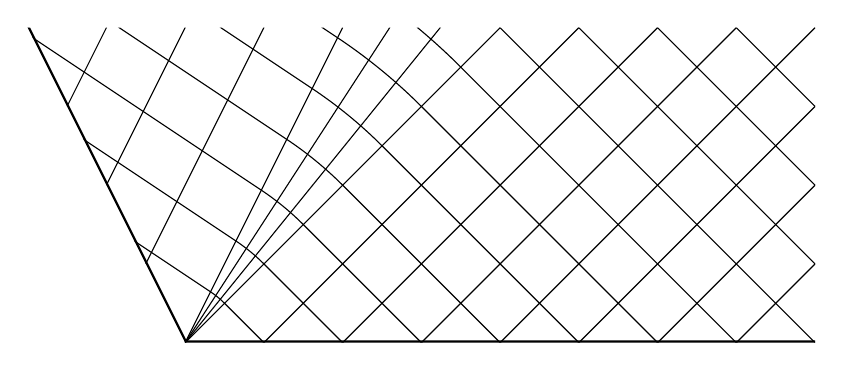
\begin{tikzpicture}
\clip (-2,4) -- (0,0) -- (8,0) -- (8,4) -- cycle;
\draw [ultra thick] (0,0) -- (8,0) (0,0) -- (-2,4);
\foreach \x in {0,...,12} {
  \draw (\x,0) -- ++(4,4) 
%        (\x,0) -- (\x/2,\x/2) arc (45:63.43:0.707*\x) -- ++(-6,4);
        (\x,0) -- (\x/2,\x/2) arc (45:56.3099:1.165*\x) -- ++(-6,4);
}
\foreach \x in {51,57} {
  \draw (0,0) -- (\x:6);
}
\foreach \y in {0,...,4} {
  \draw (-\y/2,\y) -- ++(2,4);
}
\end{tikzpicture}
\end{center}
\caption{The Characteristic Structure for a Rarefaction Wave,
  $a<0$. Notice the smooth transition between the regions.}
\end{figure}

\begin{figure}
\begin{center}
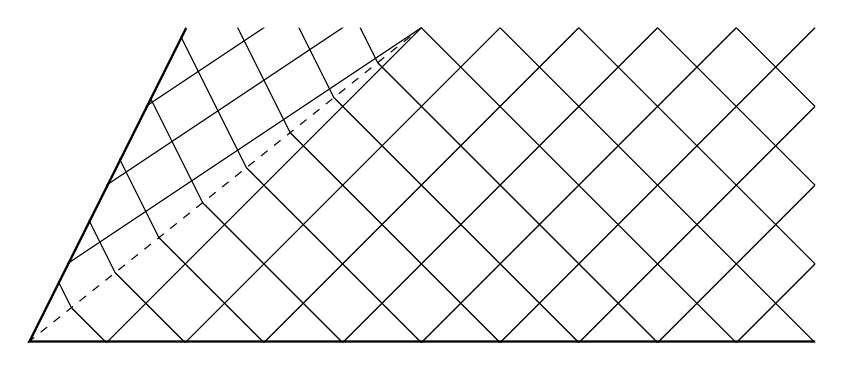
\begin{tikzpicture}
\clip (2,4) -- (0,0) -- (10,0) -- (10,4) -- cycle;
\draw [ultra thick] (0,0) -- (10,0) (0,0) -- (2,4);
\foreach \x in {1,...,14} {
  \draw (\x,0) -- ++(4,4) 
        (\x,0) -- (5*\x/9,4*\x/9) -- ++(-2,4);
}
\draw [dashed] (0,0) -- (5,4);
\foreach \y in {1,...,4} {
  \draw (\y/2,\y) -- ++(6,4);
}
\end{tikzpicture}
\end{center}
\caption{The Characteristic Structure for a Compression Wave, $a>0$. Notice the abrupt transition between the regions.}
\end{figure}

\section{Problems}
\begin{enumerate}


\item{\bf Maximum Flux}

Calculate from the Euler equation and the continuity equation, at what
velocity does the flux ($\rho V$) reach its maximum for fluid flowing 
through a tube of variable cross-sectional area?   
At which velocities does the flux vanish?  You can consider the flow
to be adiabatic.

\item{\bf Stream Bed}

  Fig.~\ref{fig:channel} shows how the level of the surface changes
  for a flow passing over an obstacle.  For an initial depth of
  $z_0=1$ and $g=10$ and a bump height of $y(x)=0.1 e^{-x^2}$, find the
  solutions to Bernoulli's equation (Eq.~\ref{eq:bern}) for $z$ as a
  function of $x$ and the initial velocity $v_0$.  You may find
  several solutions for a given $x$.   Also you should only worry
  about the positive real solutions for $z$.  What are the values of
  the critical velocities $v_0$?

\item{\bf Sound Velocity}

  Show that for a linear sound wave {\em i.e.} one in which $\delta
  \rho \ll \rho$ that the velocity $v$ of fluid motion is much less
  than $c_s$. Estimate the maximum longitudinal fluid velocity in the
  case of a sound wave in air at STP in the case of a disturbance
  which sets up pressure fluctuations of order 0.1\%.
\end{enumerate}


%%% Local Variables:
%%% TeX-master: "book"
%%% End: